\documentclass[UTF8]{ctexart}
\usepackage[a4paper,text={150true mm,224true mm},top=35.5true mm,left=30true mm,head=5true mm,headsep=2.5true mm,foot=8.5true mm]{geometry}

\usepackage{titlesec}
\usepackage{amsmath}
\usepackage{amsfonts}
\usepackage{algorithm}
\usepackage{algorithmic}
\usepackage{booktabs}


\floatname{algorithm}{算法}
\newtheorem{proposition}{命题}[section]
\newtheorem{proof}{证明}[section]
\newtheorem{theorem}{定理}[section]
\newcommand{\tabincell}[2]{\begin{tabular}{@{}#1@{}}#2\end{tabular}}

\CTEXsetup[format={\large\bfseries}]{section}  

\title{Generative Adversarial Nets\\生成式对抗网络}
\author{Ian J. Goodfellow,  Jean Pouget-Abadie, Mehdi Mirza, Bing Xu\\ David Warde-Farley, Sherjil Ozair, Aaron Courville, Yoshua Bengio\\【译】 jinxiu.qi}
\begin{document}
\maketitle
\begin{abstract}
我们提出了一种基于对抗过程的生成式估测模型框架,这个框架中,我们同时训练两个模型:一个获取数据分布的生成式模型$G$,一个估测样本来自训练数据而不是分布$G$的概率的判别式模型$D$。$G$的训练过程中,其目标是最大化$D$犯错的概率,这套框架就如同极大-极小的双方博弈。对于任意函数$G$和$D$的空间中,当$G$找到了训练数据的分布,并且$D$处处等于$\frac{1}{2}$时,意味着该解为唯一解。在$G$和$D$都用多层感知器定义时,整个系统可以通过反向传播进行训练。在训练或生成样本的过程中,不需要使用网络近似推理或者马尔可夫链,实验揭露了这套框架在生成样本上质和量的潜力。
\end{abstract}

\section{导言}
自己去看论文,不翻了。
\section{相关工作}
自己去看论文,不翻了。
\section{对抗网络}
当模型都是多层感知器时,对抗模型很容易实现。为了学习数据$x$上分布$p_g$的样本生成器,我们定义一个先验变量$p_z(z)$作为数据空间映射$G(z;\theta_g)$的噪声输入,其中$G$是由参数$\theta_g$确定的多层感知器所表达的可微函数。我们还需要定义一个输出标量的多层感知器$D(x;\theta_d)$,$D(x)$代表$x$是来自数据而不是$p_g$的概率。训练$D$时,我们最大化正确地给数据样本和生成样本贴标签的概率,我们同时训练$G$使得它最小化$\log(1 - D(G(z)))$,换言之,$D$和$G$进行下面这个函数$V(G, D)$所表示的极大-极小双方博弈:
\begin{equation}\label{equ: minmax}
\min\limits_{D}\max\limits_{G}V(G, D) = \mathbb{E}_{x\sim p_{data}(x)}[\log D(x)] + \mathbb{E}_{x\sim p_{z}(x)}[\log(1-D(G(z))]
\end{equation}

下一小节中,我们对对抗网络的理论分析基本上表明,训练这个准则可以寻找到数据的生成分布$G$,并且$D$得到一个较好的性能。图\ref{img: figure}是一种对这套方法的非正式而易懂的解释。实际中,我们必须通过一个迭代的数值逼近来实现这种博弈。在训练的内循环中最优化$D$是一个高代价的计算,并且在有限数据集中会导致过拟合。相反的,我们轮换地进行$k$次最优化$D$以及1次最优化$G$。只要$G$的变动足够小,便能确保$D$维持在它的最优解附近,整个过程的正式描述如算法\ref{alg1}所示。

工程上,式\eqref{equ: minmax}可能无法为$G$提供足够的梯度,在学习的早期,$G$还很弱鸡,$D$却很强势,因为$G$生成的样本与训练数据差太多了, $D$有足够的置信度做出决策,此时$\log(1-D(G(z)))$进入饱和。因此我们通过最大化$\log D(G(z))$来训练$G$而不是最小化$\log(1-D(G(z)))$,这两个目标函数都会使得$G$和$D$收敛到相同的点,但前者可以在训练早期中提供更强的梯度。

\begin{algorithm}
\caption{生成式对抗网络的小批量随机梯度下降训练算法。判别器的训练次数$k$为一个超参数,在实验中,我们使用计算负载最小的选项,即$k=1$。} 
\label{alg1}       
\begin{algorithmic} 
\FOR{number of training iterations}
\FOR{$k$ steps}
\STATE 从噪声先验$p_g(z)$中采样出$m$个噪声样本$\{z^{(1)}, \cdots, z^{(m)}\}$
\STATE 从数据分布$p_{data}(x)$中采样出$m$个样本$\{x^{(1)}, \cdots, x^{(m)}\}$
\STATE 使用梯度上升更新判别器参数
\begin{equation*}
\Delta_{\theta_d}\frac{1}{m}\sum\limits_{i=1}^m[\log D(x^{(i)}) + \log(1 - D(G(z^{(i)})))]
\end{equation*}
\ENDFOR
\STATE 从噪声先验$p_g(z)$中采样出$m$个噪声样本$\{z^{(1)}, \cdots, z^{(m)}\}$
\STATE 使用梯度下降更新生成器参数
\begin{equation*}
\Delta_{\theta_g}\frac{1}{m}\sum\limits_{i=1}^m \log(1 - D(G(z^{(i)})))
\end{equation*}
\ENDFOR
\STATE 参数更新可以使用任何一种标准的基于梯度的学习算法,我们在实验中在加入动量项。
\end{algorithmic}
\end{algorithm}



\begin{figure}[htbp]
\begin{center}
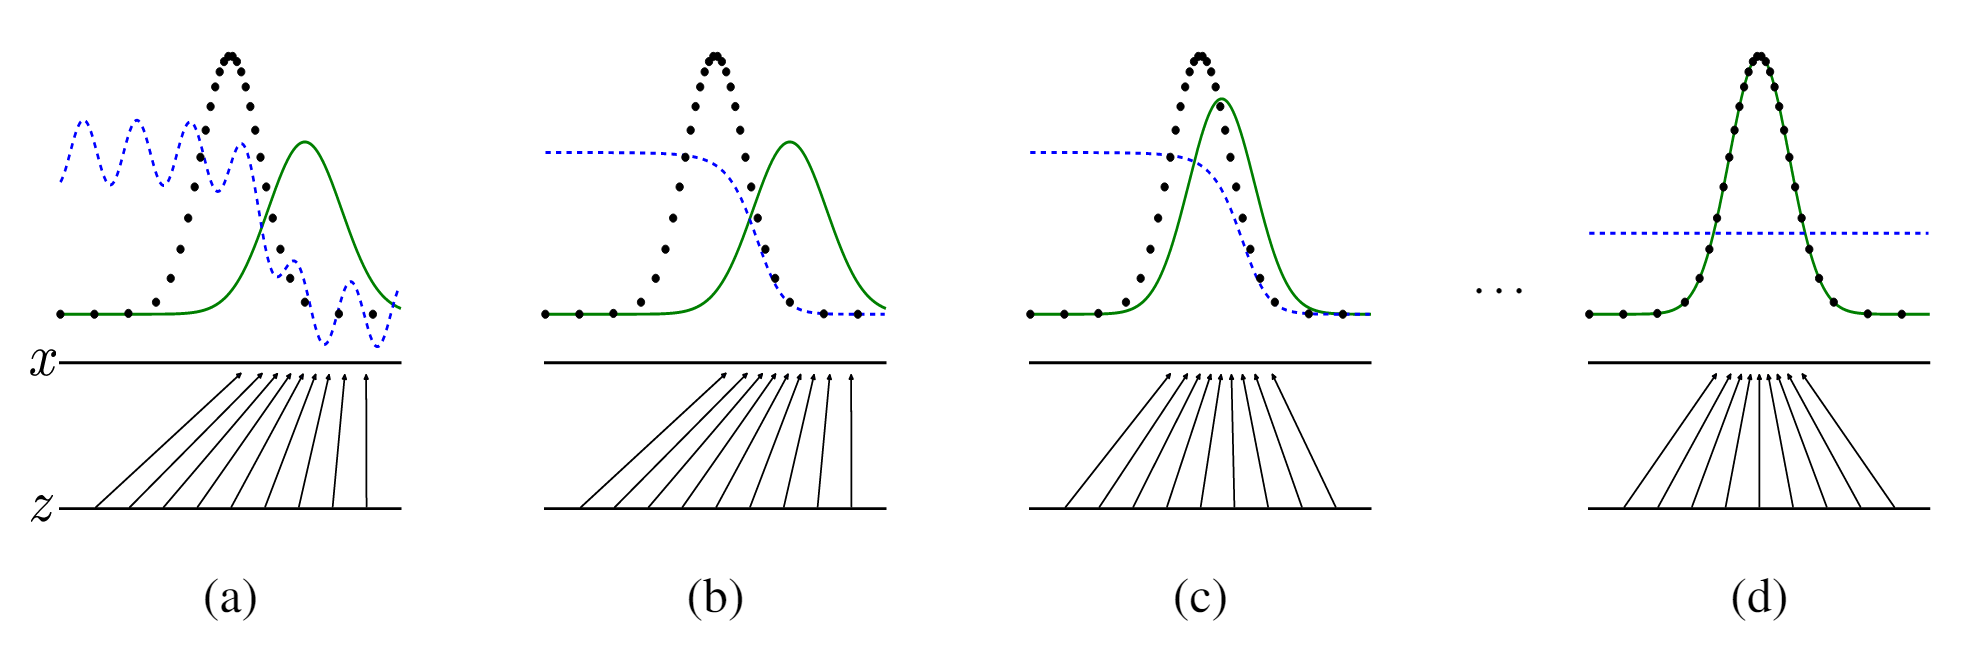
\includegraphics[width=0.9\linewidth]{image/figure.png}
\end{center}
\caption{生成式对抗网络的训练过程中,同时地更新判别式分布$D$(蓝色虚线),使得它可以辨析生成式分布$p_g(G)$(绿色实线)和数据分布(黑色点线)。平行线中,下面一条为$z$的采样域,这个例子中的是均匀分布,对应的,平行线上面一条为$x$的一部分域。向上指着的箭头说明映射$x = G(z)$如何通过样本转换得到非均匀分布的分布$p_g$。$G$在$p_g$的高密度区域收缩,并低密度区域扩张。(a)对抗组近乎收敛的情况:$p_g$与$p_{data}$相似,并且$D$是一个准确率特别高的分类器。(b)在算法的内循环中,训练$D$用于判别样本是否来源于数据,最后会收敛于$D^*(x)=\frac{p_{data}(x)}{p_{data}(x) + p_g(x)}$。(c)当对$G$执行完一个更新后,$D$的梯度引导$G(x)$往使得样本更容易被判定为数据样本的区域滑动。(d)经过几个训练周期,如果他们获取到足够的性能,那么他们将到达一个无法再提升的点,因为此时$p_g = p_{data}$,判别器将无法区分这两个分布,也就是说,$D(x) = \frac{1}{2}$}
\label{img: figure}
\end{figure}



\section{理论分析}
生成器$G$隐式地定义了一个概率分布$p_g$作为从$z\sim p_z$中获取样本$G(z)$的样本分布。因此,我们希望在足够多的资源和时间时,算法\ref{alg1}收敛到$p_{data}$的一个较好的估计上。本节中,我们基于非参环境进行讨论,换言之,我们讨论拥有无穷资源的模型在概率密度函数空间中的收敛性。我们在章节\ref{sec:4.1}中说明极大极小博弈的优化目标$p_g=p_{data}$存在全局最优解,随后的章节\ref{sec:4.2}中,我们会讨论优化式\eqref{equ: minmax}的算法\ref{alg1}可以使得我们获取到这个最优解。

\subsection{全局优化目标$p_g = p_{data}$\label{sec:4.1}}
我们首先考虑任意一个给定的生成器$G$下的最优判别器$D$。
\begin{proposition}
对于给定的$G$,最优判别器$D$为
\begin{equation}
D^*_G(x)=\frac{p_{data}(x)}{p_{data}(x) + p_g(x)} \label{equ:Optimal}
\end{equation}
\end{proposition}
\begin{proof}
对于任意给定的生成器$G$,判别器$D$的训练准则为最大化$V(G, D)$
\begin{equation}
\begin{split}
V(G, D) &= \int_x p_{data}(x)\log(D(x))dx + \int_z p_z(z)\log(1 - D(g(z))dz\\
&= \int_x p_{data}(x)\log(D(x)) + p_g(x)\log(1 - D(x))dx
\end{split}
\end{equation}
对于任意的$(a, b)\in \mathbb{R}^2 \setminus \{0, 0\}$,函数$y \rightarrow a\log(y) + b\log(1-y)$在区间$[0, 1]$上的$\frac{a}{a+b}$获取其最大值,并且判别器不需要在$Supp(p_{data}) \cup Supp(p_g)$的外部定义。证毕。
\end{proof}

另一方面,$D$的训练目标可以视为最大化条件概率$P(Y=y|x)$估计的对数似然,其中,$Y$指明$x$是来自$p_{data}$(此时$y=1$)还是来自$p_g$(此时$y=0$)。式\eqref{equ: minmax}所代表的极大极小博弈现在重新解释为
\begin{equation}\label{equ:CG}
\begin{split}
C(G) &= \max\limits_D V(G, D)\\
&= \mathbb{E}_{x\sim p_{data}}[\log D_G^*(x)] + \mathbb{E}_{z\sim p_z}[\log(1 - D_G^*(G(z)))]\\
&=\mathbb{E}_{x\sim p_{data}}[\log D_G^*(x)] + \mathbb{E}_{z\sim p_g}[\log(1 - D_G^*(x))]\\
&=\mathbb{E}_{x\sim p_{data}}[\log \frac{p_{data}(x)}{p_{data}(x) + p_g(x)}] + \mathbb{E}_{z\sim p_g}[\log\frac{p_g(x)}{p_{data}(x) + p_g(x)}]
\end{split}
\end{equation}

\begin{theorem}\label{the:1}
虚拟的训练准则$C(G)$当且仅当$p_g = p_{data}$时取得全局最小值$-\log 4$
\end{theorem}
\begin{proof}
由式\eqref{equ:Optimal}可知,对于$p_g = p_{data}$有$D_G^*(x) = \frac{1}{2}$,代入式\eqref{equ:CG}得$C(G) = \log \frac{1}{2} + \log	\frac{1}{2} = -\log 4$。下面证明充要性,首先观察
\begin{equation*}
\mathbb{E}_{x\sim p_{data}}[-\log 2] + \mathbb{E}_{x\sim p_g}[-\log 2] = -\log 4
\end{equation*}

然后我们用$C(G)=V(D^*_G, G)$减去这个上面这个数值\footnote{译注:其实就是将$V(D^*_G, G)$转换成KL散度形式,为了使得等式成立,需要减去$\log 4$},我们将得到
\begin{equation}
C(G) = -\log 4 + KL\Big(p_{data} \Big|\Big| \frac{p_{data} + p_g}{2} \Big) + KL\Big(p_g \Big|\Big| \frac{p_{data} + p_g}{2}\Big)
\end{equation}
式中,$KL$为KL散度\footnote{译注:或称相对熵,定义为$KL(P||Q) = \sum\limits_i P(i)\log\frac{P(i)}{Q(i)}$}(Kullback–Leibler divergence),我们将这个等式化简为模型分布和生成分布这两个分布的JS距离\footnote{译注:根据对称性定义出的一种距离,$JSD(P || Q) = \frac{1}{2}KL(P || M) + \frac{1}{2}KL(Q || M)$,其中$M = \frac{1}{2}(P+Q)$}(Jensen Shannon divergence)
\begin{equation}
C(G) = -\log 4 + 2 \cdot JSD(p_{data} || p_g)
\end{equation}
因为两个分布间的JS距离是非负的,当且仅当两者相等的时候取的最小值0,因此全局最小值$C^*=-\log 4$的唯一解在$p_g = p_{data}$时取到,即生成式模型可以完美地取代数据分布的时候。
\end{proof}

\subsection{算法\ref{alg1}的收敛性\label{sec:4.2}}

\begin{proposition}
如果在算法\ref{alg1}的每个迭代中,$G$和$D$拥有足够多的资源,给定$G$的情况下,判别器会收敛到它的最优解,并且,为了最大化准则
\begin{equation*}
\mathbb{E}_{x\sim p_{data}}[\log D_G^*(x)] + \mathbb{E}_{z\sim p_g}[\log(1 - D_G^*(x))]
\end{equation*}
$p_g$会更新至收敛于$p_{data}$。
\end{proposition}
\begin{proof}
正如上面提到的准则,定义一个$p_g$的函数$V(G, D) = U(p_g, D)$,不难看出$U(p_g, D)$是$p_g$的一个凸函数。凸函数的上确界的次导数包含了该函数在最大值处的导数,换言之,如果$f(x) = \sup_{\alpha\in \mathcal{A}}f_\alpha(x)$,并且对于所有的$\alpha$,$f_\alpha(x)$都是$x$的凸函数,那么如果$\beta = \arg\sup_{\alpha\in\mathcal{A}}f_\alpha(x)$,则有$\partial f_\beta(x) \in \partial f$。这等价于在给定的$G$所对应的最优的$D$中,对$p_g$使用梯度下降更新规则。定理\ref{the:1}中我们证明了$p_g$的凸函数$\sup_DU(p_g, D)$存在唯一的全局最优解,因此对$p_g$使用足够小的更新步长,$p_g$将收敛于$p_x$,证毕。
\end{proof}

实际中,通过函数$G(z;\theta_g)$,对抗网络只能描述分布$p_g$的有限族,并且我们优化$\theta_g$而不是$p_g$自身,所以证明并适用于实际。然而,工程中多层感知器网络杰出的性能表明,尽管缺乏理论的保证,它们依然是十分靠谱的模型。
\section{实验}
自己去看论文,不翻了。
\section{优缺点}
相对于现有的模型框架,这套新的框架有其自身的优缺点。最大的缺点在于,$p_g(x)$没有一个明确的表达式,并且在训练中,$G$和$D$必须要保证同步(特别的,$G$不能在$D$没怎么训练的情况下训练得太过火,防止出现the helvetica scenario现象\footnote{译注:一个纯搞笑冷笑话伪科普剧look around you第一集的梗......youtube上有完整的第一集},即$G$使得$z$中大部分的值与$x$一样,以至缺乏多样性)。优点在于,这里不需要马尔可夫链,只需要反向传播以获取梯度,训练过程中,推断也不需要,并且,很多函数可以整合到模型中去。表\ref{tbl:1}对生成式对抗网络与其他生成式模型做了一个汇总对比。

\begin{table}[!hbp]
\begin{center}
\begin{tabular}{ccccc}
\toprule
    & 深度有向图模型 & 深度无向图模型 & 生成式自编码机 & 对抗模型 \\
\midrule
训练 & 需要推断 & \tabincell{c}{需要推断,需要\\MCMC逼近配\\分函数梯度 }& \tabincell{c}{需要权衡重构生\\成器的mixing\\和power} & \tabincell{c}{需要同步生成器\\和判别器} \\
推断 & 近似推断 & 变分推断 & 基于MCMC推断 & 近似推断 \\
采样 & 毫无压力 & 需要马尔可夫链 & 需要马尔可夫链 & 毫无压力 \\
评估$p(x)$ & \tabincell{c}{比较困难,可通\\过AIS近似} & \tabincell{c}{比较困难,可通\\过AIS近似}  &  \tabincell{c}{没有明确表达式,\\可通过Parzen估计} & \tabincell{c}{没有明确表达式,\\可通过Parzen估计} \\
模型设计 & \tabincell{c}{模型要能在推断\\scheme下运作} & \tabincell{c}{需要细心设计很\\多个属性}& \tabincell{c}{理论上只要可微\\的函数都可以}& \tabincell{c}{理论上只要可微\\的函数都可以} \\
\bottomrule
\end{tabular}
\caption{生成式模型\label{tbl:1}}
\end{center}

\end{table} 

前面讲的优点主要在于计算方面,在统计方面,生成式对抗网络的优点在于它不直接地通过数据样本进行更新,而是通过判别器灌回来的的梯度更新,这也就意味着,输入的组成原件并不直接的复制到生成器的参数中,另一个优点在于,这种网络可以描述大尖峰,甚至是退化分布,而基于马尔可夫链的方法,为了让链能够将模型混合,需要保证分布有一定程度的模糊。




\section{结论与展望}
自己去看论文,不翻了。
\end{document}